\documentclass[12pt,a4paper]{article}
\usepackage[marginparsep=8pt,left=2.5cm,right=2.5cm,top=2.5cm,bottom=3cm]{geometry}
\usepackage{graphicx}
\usepackage[utf8]{inputenc}
%\setlength{\parindent}{0pt}% Remove paragraph indent
\graphicspath{ {./images/} }

\begin{document}

\title{\LARGE \bf Domácí úkol na BI-PST 2018}
 \author{Pavel Jahoda a Jan Lidák}

\maketitle

\section{Střední hodnota, rozptyl, medián}
Data jsou z pozorování 59 vrabců během zimy. První veličina {\bf X} reprezentuje váhy vrabců v gramech. Druhá veličina {\bf Y} nabývá dvou hodnot 'survived', pokud vrabec přežil a 'perished' pokud nepřežil. Sledovanou proměnnou X jsme rozdělili na dvě pozorované skupiny {\bf X1} (vrabci co přežili) a {\bf X2} (vrabci co nepřežili).\\
EX1=25.463, var(X1)=1.539 a medián je 25.7.\\
EX1=26.275, var(X2)=2.078 a medián je 26.\\
\par \bigskip

\section{Distribuční funkce}
Jako nejbližší rozdělení pro váhu vrabců se nabízí normální rozdělení. Přežití vrabců zato vypadá na Bernoulliho rozdělení.\\

\section{Generovaný výběr}
Na následujících grafech je zobrazeno 100 vygenerovaných hodnot dle normálního rozdělení s parametry $\lambda$ = EX = 25.793 a $\sigma ^2$ = varX = 1.918. Bernoulliho rozdělení s p = 0.593.

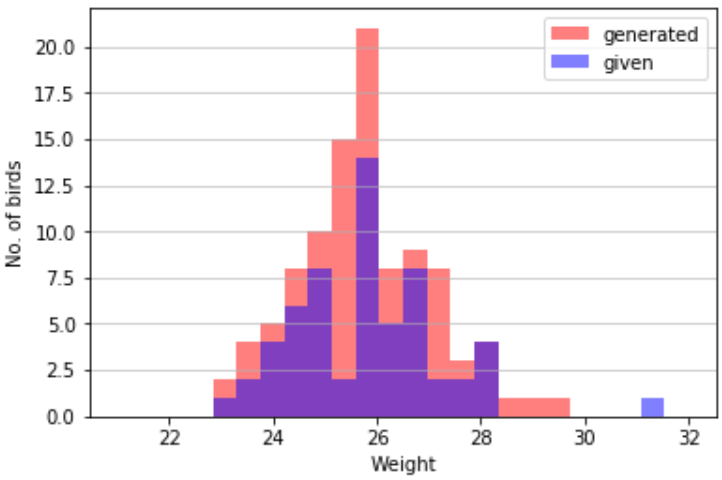
\includegraphics[scale=0.31]{gen_weight_graph2}
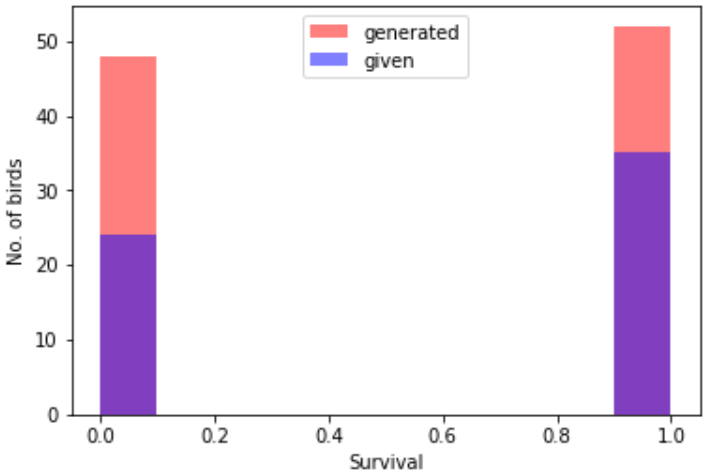
\includegraphics[scale=0.31]{gen_survival_graph2}

Data mají 59 záznamů, přišlo nám tedy příhodné vygenerovat i stejný počet, aby byla lépe vidět podobnost námi vybraných rozdělení a původní datové množiny.

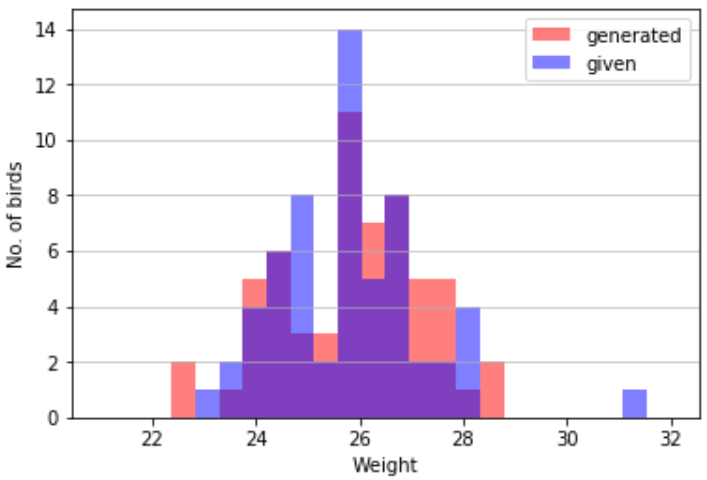
\includegraphics[scale=0.31]{gen_weight_graph1}
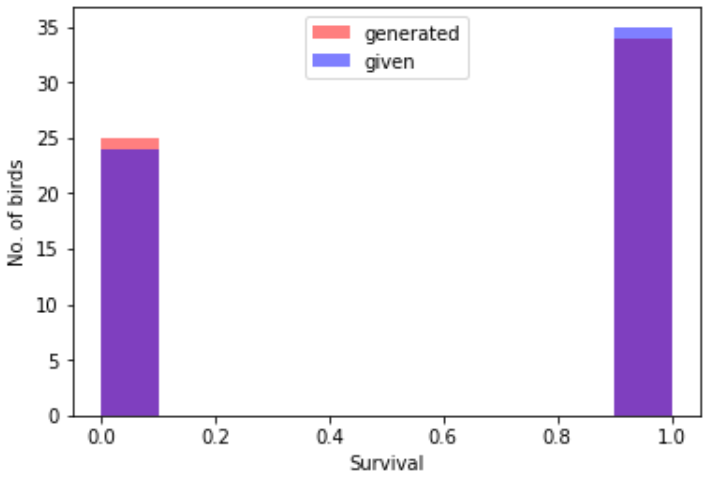
\includegraphics[scale=0.31]{gen_survival_graph1}
\par \bigskip


\end{document}

